\documentclass[oneside,a4paper,12pt]{memoir}
\usepackage{amssymb,amsmath}
\usepackage{chngcntr}
\usepackage{color}
\usepackage[latin1]{inputenc}
\usepackage[ruled,vlined,linesnumbered]{algorithm2e}
\usepackage{graphicx}
%\usepackage{caption}
\usepackage{subcaption}
\usepackage{url,hyperref}
\usepackage{booktabs}
\usepackage{float}
\usepackage{colortbl}
\usepackage{comment}
\usepackage{ulem}
\usepackage{todonotes}

\begin{document}
\title{SAIM - Manual}
\author{Klaus Lyko}                                                  
\maketitle

\chapter{Introduction}
Links between instance are of central importance for the Semantic Web and for a large number of tasks, such as data integration, federated querying and knowledge retrieval. Finding those links is the subject of Link Deiscovery (LD).
Two main problems arise when trying to discover links between datasets.

First, naive solutions have to compare all instances of a source knowledge base with all instances of the target knowledge base, thus having a quadratic time complexity. Second, one have to guarantee the quality of those links. 
To address the first problem time efficient algorithms and frameworks such as SILK\footnote{\url{https://www.assembla.com/spaces/silk/}} and LIMES\cite{NGAU11} have been developed to reduce the number of comparisons. For the second problem both supervised (e.g. \cite{NGLY12, NGO+13}) and unsupervised ({e.g. \cite{NIK+12}}) machine learning approaches have been developed.

SAIM \footnote{SAIM stands for (\uline{S}emi-)\uline{A}utomatic \uline{I}nstance \uline{M}atcher.}  encompasses solutions for both problems within one interface. It is based upon algorithms implemented in the LIMES\footnote{\url{http://limes.sf.net/}} framework which have been shown to outperform state-of-the-art in previous work w.r.t. time-complexity \cite{NGON12c}. SAIM offers an intuitive GUI for experts to manually create Link Specifications while implementing the supervised and unsupervised machine learning algorithms EAGLE \cite{NGLY12}	and COALA \cite{NGO+13} respectively, which have been shown to lead to highly accurate link specifications.

This manual will cover the complete workflow of SAIM. Starting in chapter \ref{kbdefinition} from scratch it will cover the process of defining the endpoints(\ref{endpoint}), class restrictions(\ref{classes}) and properties(\ref{properties}) of the knowledge bases to link. Chapter \ref{manual} describes how experts can build link specifiactions manually. Chapter \ref{selfconfig} and \ref{learning} discusses the unsupervised and supervised learning algorithms respectively. Finally, chapter \ref{features} covers additional features of SAIM such as saving and loading link specifications, uploading RDF dumps.

%%%%%%%%%%%%%%%%%                                  ENDPOINTS 													%%%%%%%%%%%%%%%%%%%%%%%%%
\chapter{Source and Target Endpoint definition}
\label{kbdefinition}
	Upon start SAIM 
	\begin{figure}
		\centering
		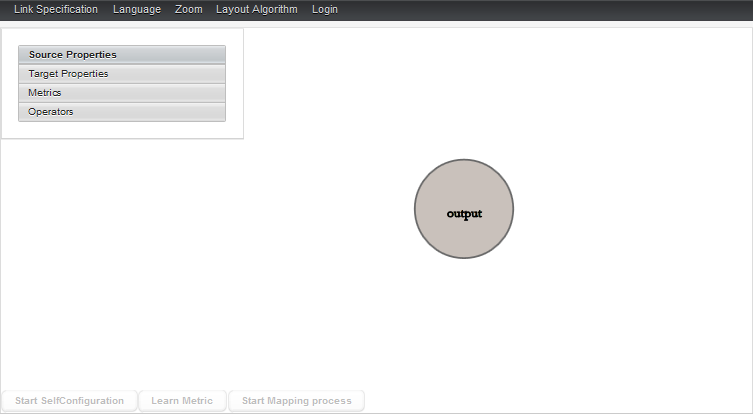
\includegraphics[width=\textwidth]{images/main.png}
		\caption{Main Window}
		\label{fig:MainWindow}
	\end{figure}
	

	\todo{Write something}
	\section{Endpoints}
	\label{endpoint}
	 \subsection{Presets}
	\section{Class restriction}
	\label{classes}
	\section{Property Matching}
	\label{properties}
%%%%%%%%%%%%%%%%                              MANUAL LINK SPECS 											%%%%%%%%%%%%%%%%%%%%%%%%%
\chapter{Manual metric definition and execution}
\label{manual}

%%%%%%%%%%%%%%%%%                             SELFCONFIGURATION 											%%%%%%%%%%%%%%%%%%%%%%%%%
\chapter{Selfconfiguration}
\label{selfconfig}

%%%%%%%%%%%%%%%%%                                  LEARNING 													%%%%%%%%%%%%%%%%%%%%%%%%%
\chapter{Improving results through learning}
\label{learning}

%%%%%%%%%%%%%%%%%                                  FEATURES 													%%%%%%%%%%%%%%%%%%%%%%%%%
\chapter{Additional features}
\label{features}

\bibliographystyle{plain}
\bibliography{saim}

\end{document}